\documentclass[10pt, uplatex, dvipdfmx]{jsarticle}
\usepackage{../mypackage}

\graphicspath{{../pictures}}

\setcounter{section}{9}

\begin{document}

\section{広義2重積分}

有界閉領域とは限らない集合上の有界とは限らない関数の2重積分を定義する.

\subsection{増加近似列}

有界閉領域でない集合 $D$ 上の2重積分は,$D$ に近づく有界閉領域上の2重積分
の極限として定義する.そこで,まず「集合 $D$ に近づく」ということを正確
に定義する.

\begin{definition}
  $D \subset \mathbb{R}^2$ に対し,以下を満たす有界閉領域の
  列 $\Set{D_n}$ を $D$ の\textbf{増加近似列}という.
  \begin{enumerate}[(1)]
  \item
    $D_1 \subset D_2 \subset \cdots \subset D_n \subset D_{n+1}
    \subset \cdots \subset D$
  \item 任意の有界閉領域 $K \subset D$ に対して,十分大きな自然数 $n$
    を選べば $K \subset D_n$ となる.
  \end{enumerate}  
\end{definition}

\begin{example}\label{ex:Lopen}
  自然数 $n$ に対して($D_n$ に関しては $n \geqq 2$ とする)
   \begin{align*}
     D_n = \left[ \frac{1}{n}, 1\right] \times [0,1], \quad E_n=\left[e^{-n}, 1\right] \times [0,1]
  \end{align*}
   とすると,$\Set{D_n}$ と $\Set{E_n}$ はいずれも $D=(0,1] \times [0,1]$ の増加
    近似列である.
  \begin{figure}[h]
    \centering
    \begin{tabular}{cc}
      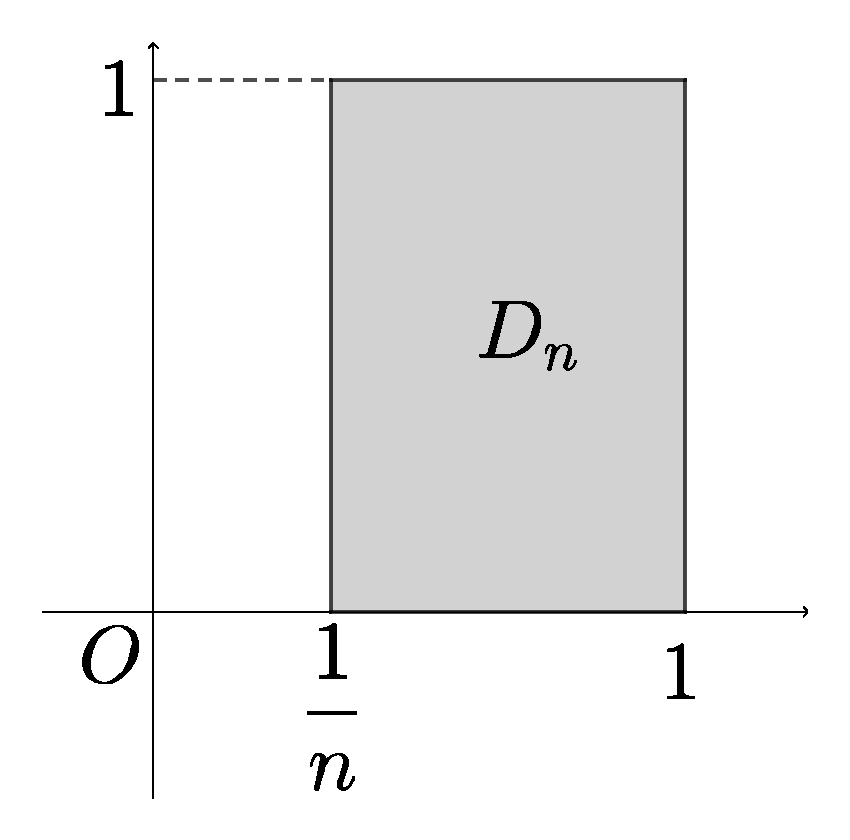
\includegraphics[height=4cm]{10/Lopen1.pdf}
      & 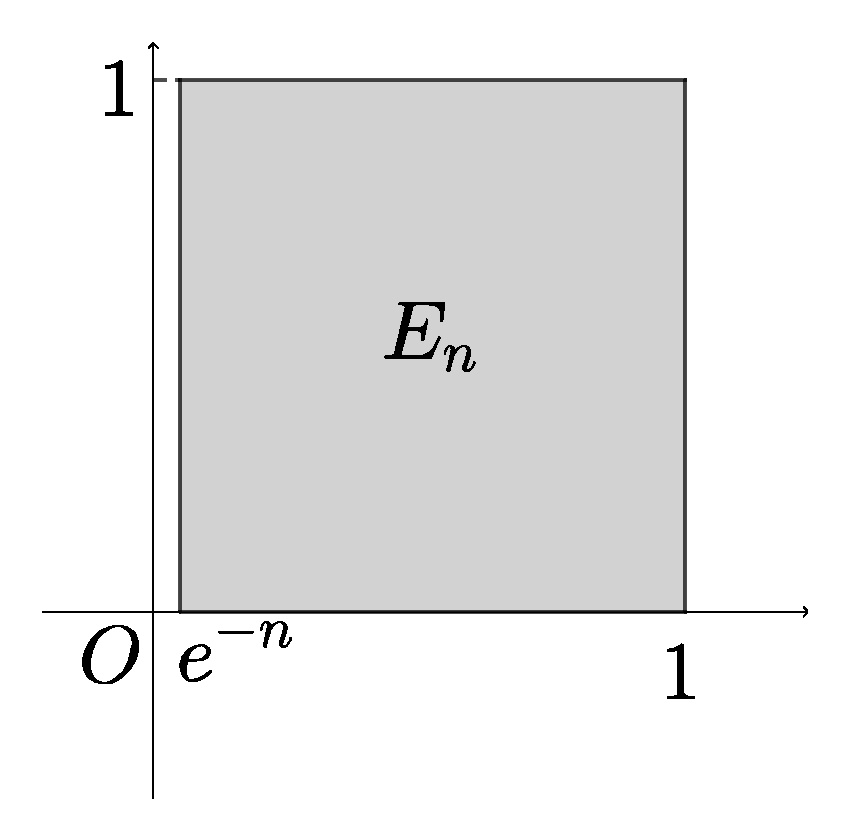
\includegraphics[height=4cm]{10/Lopen2.pdf}\\
    \end{tabular}
  \end{figure}
\end{example}

\begin{example}
  自然数 $n$ に対して
  \[
    D_n = [-n, n] \times [-n,n], \quad E_n=\Set{(x,y) | x^2+y^2 \leq n^2}
  \]
  とすると,$\Set{D_n}$ と $\Set{E_n}$ はいずれも $\mathbb{R}^2$ の増加近似列である.
  \begin{figure}[h]
    \centering
    \begin{tabular}{cc}
      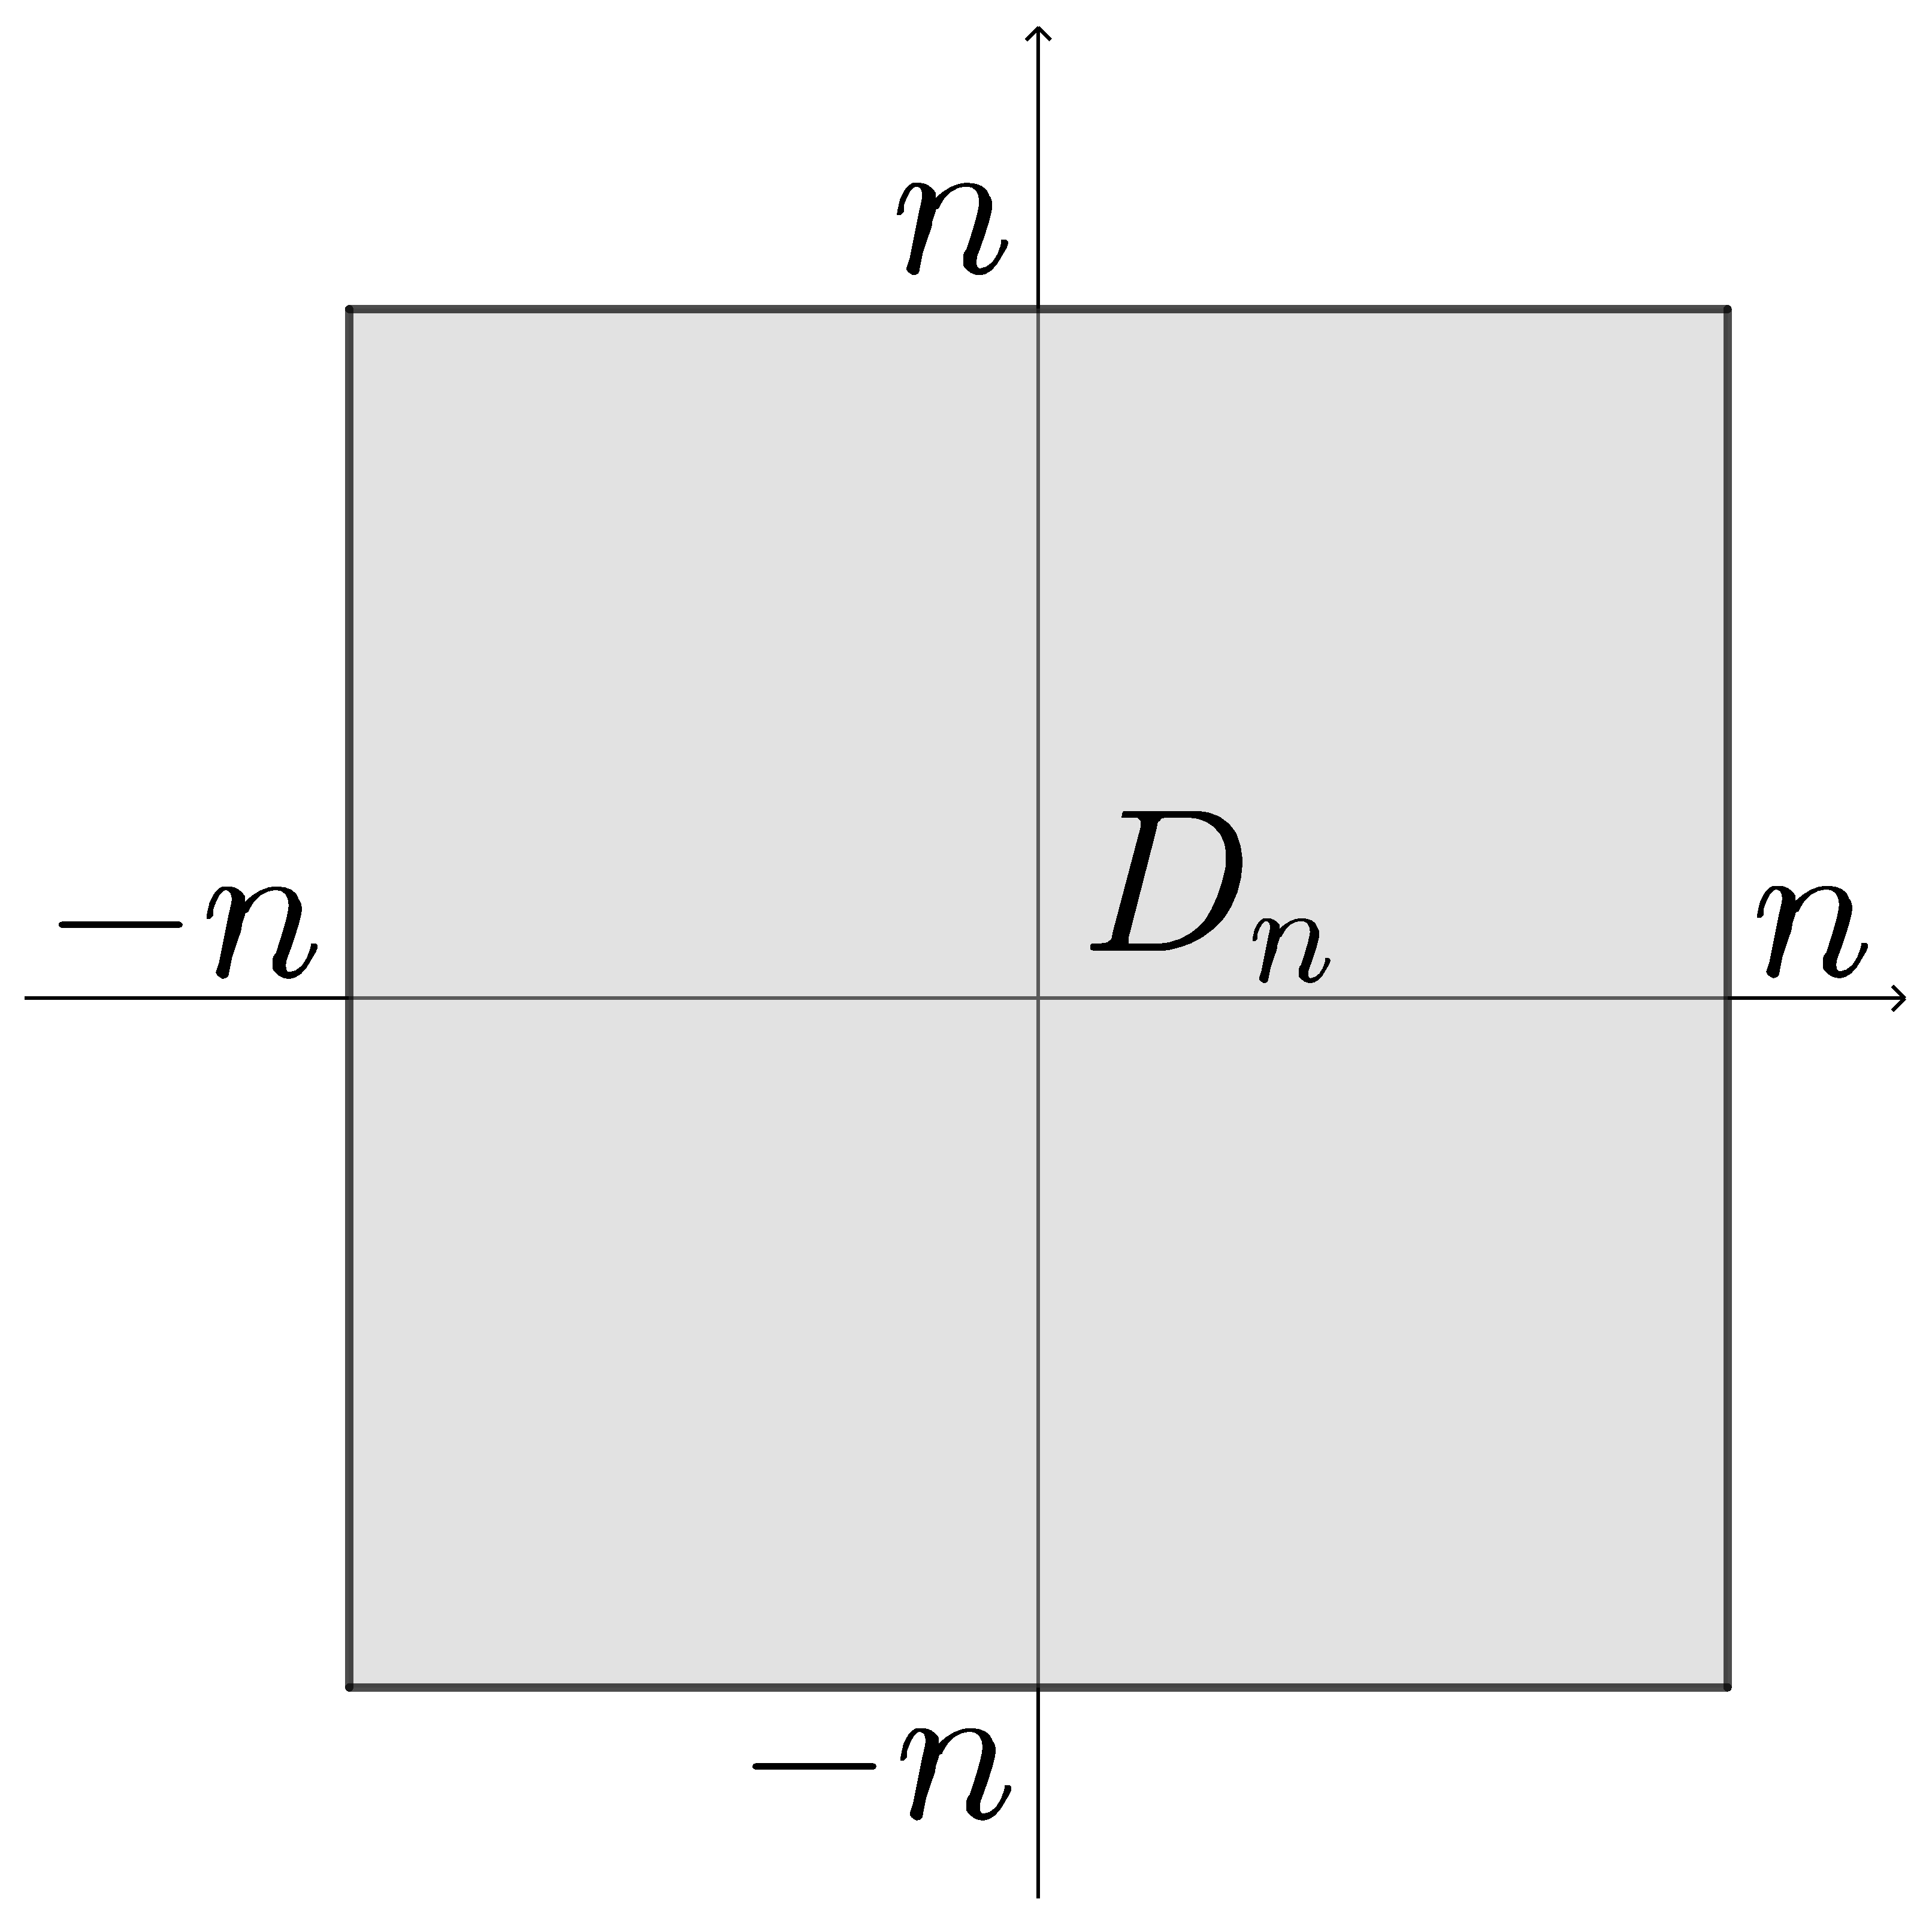
\includegraphics[height=4cm]{10/Infplane1.pdf}
      & 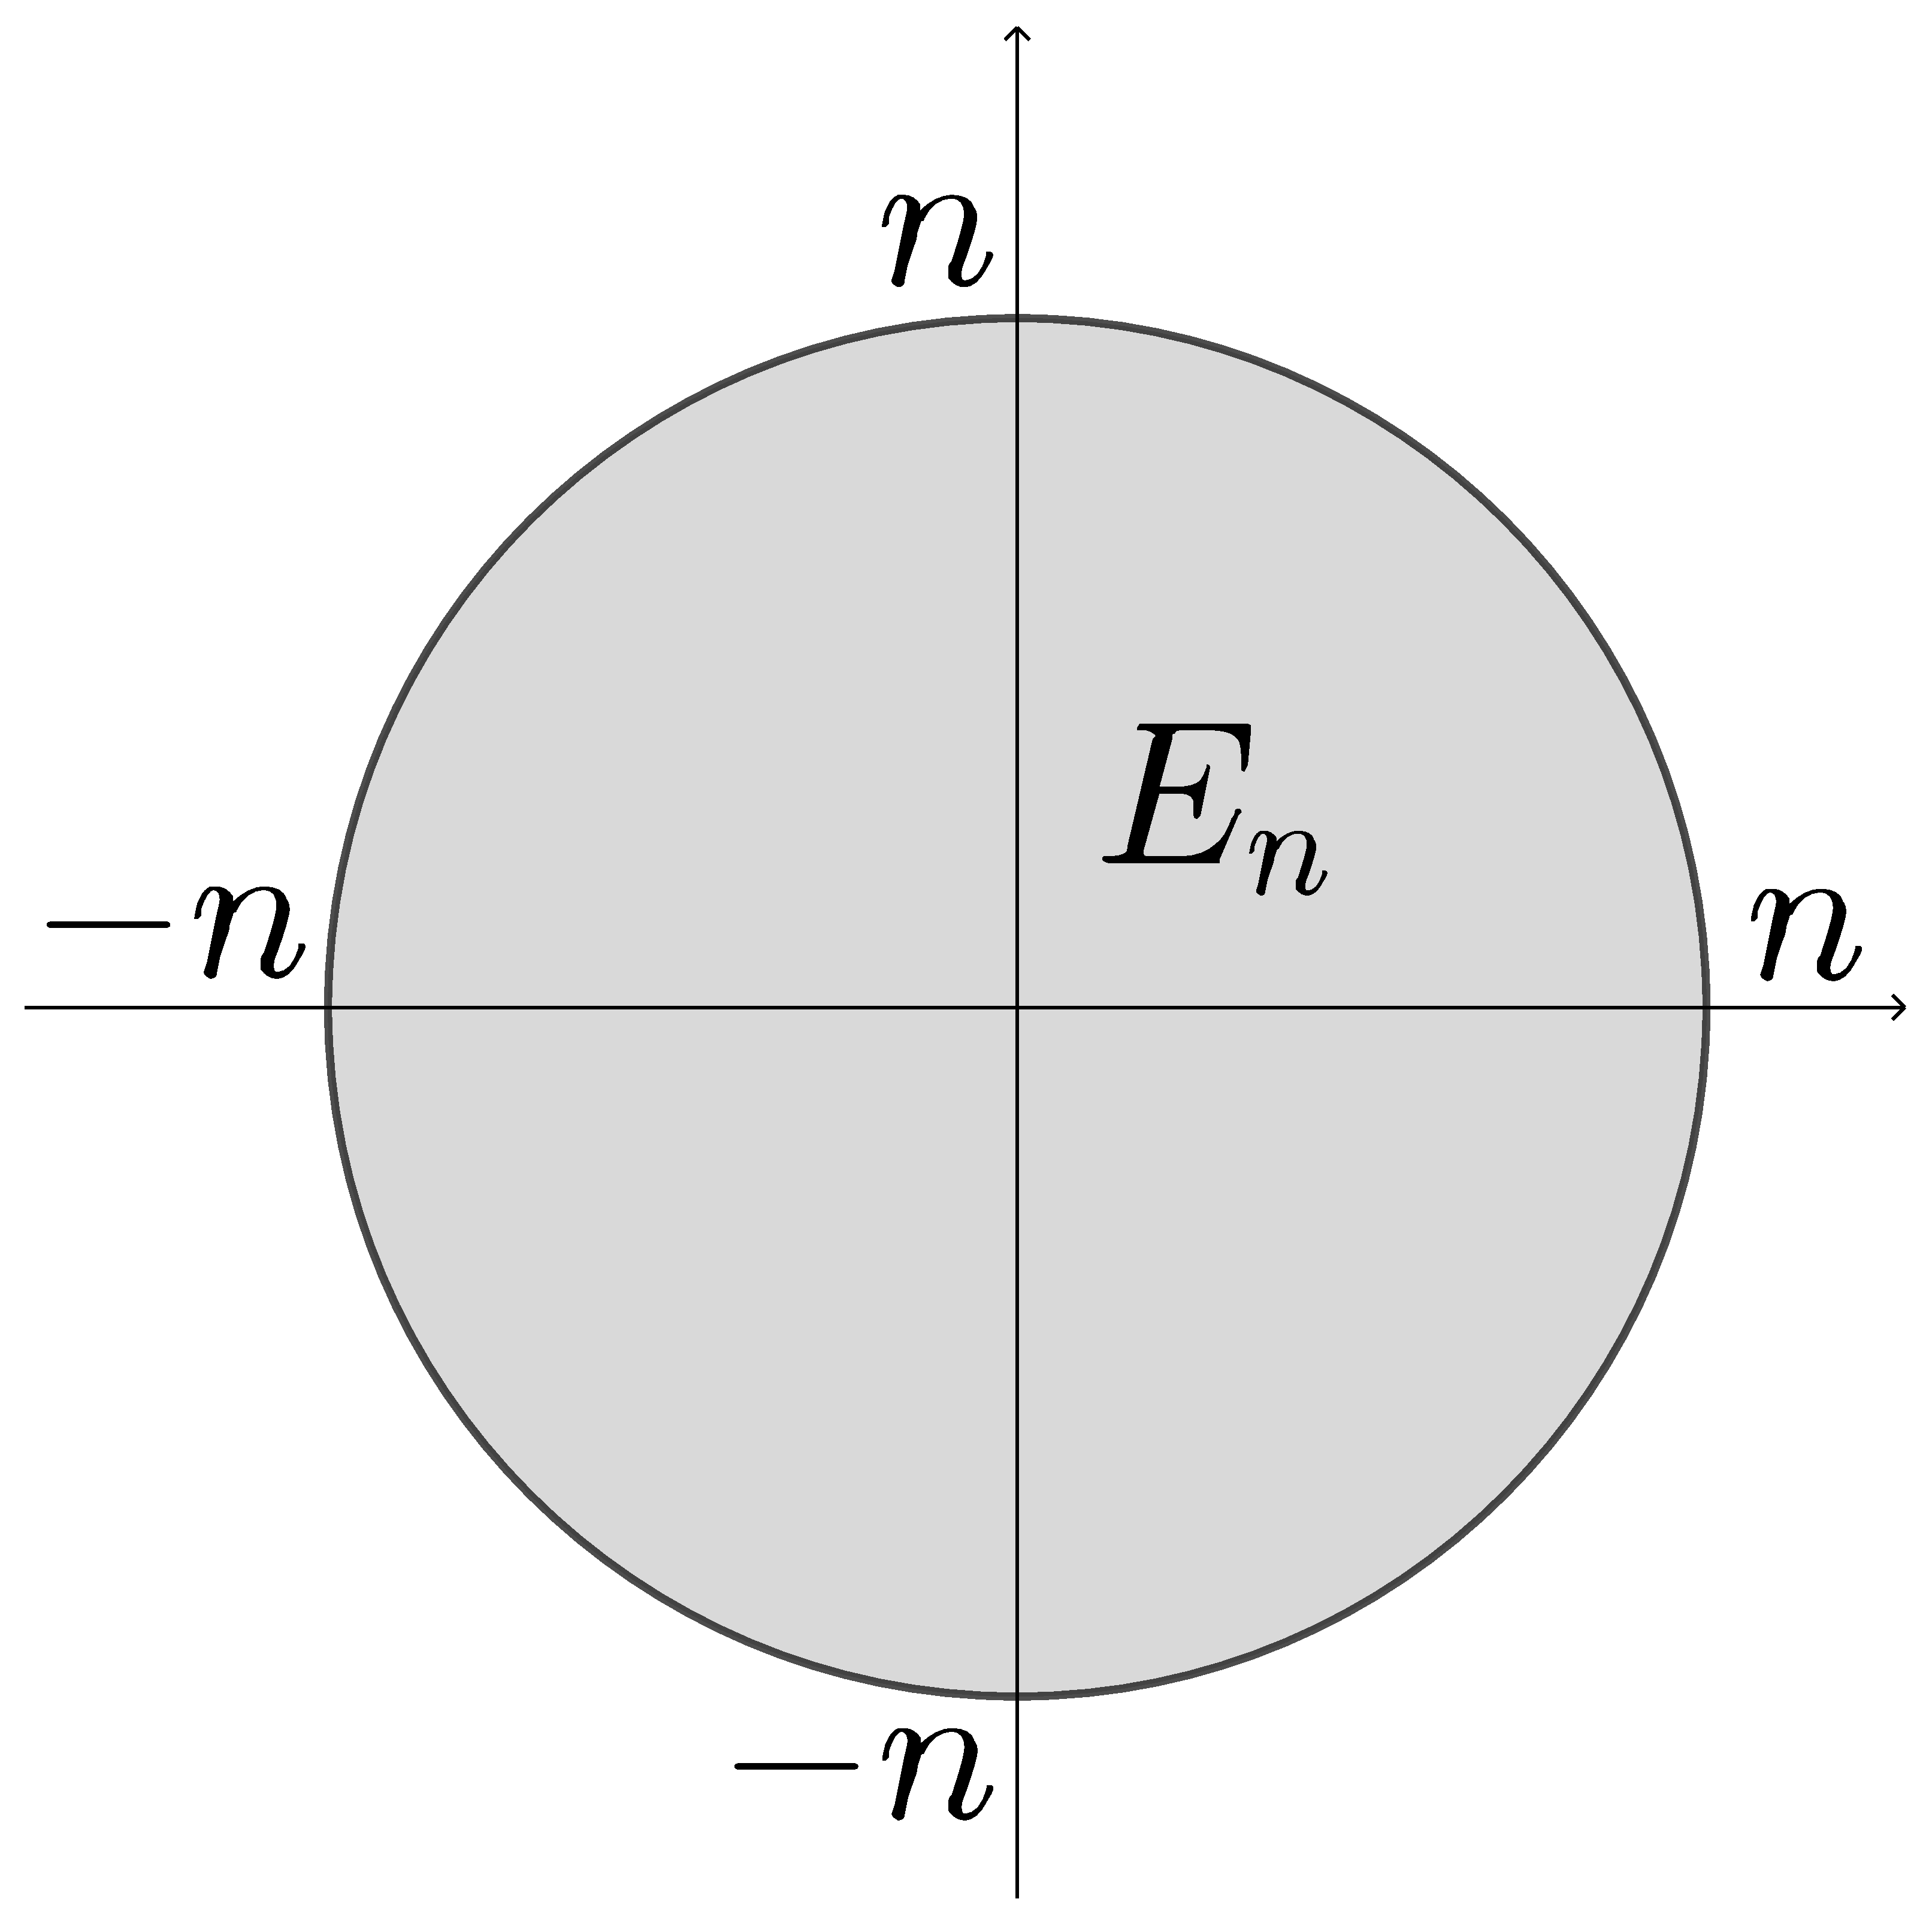
\includegraphics[height=4cm]{10/Infplane2.pdf}
    \end{tabular}
  \end{figure}
\end{example}

\subsection{広義2重積分の定義}

\begin{definition}
  $f$ を $D \subset \mathbb{R}^2$ 上定義された2変数関数とし,$D$ に含ま
  れる任意の有界閉領域上有界とする.このとき,$D$ のどんな増加近似
  列 $\Set{D_n}$ に対しても $f$ が各 $D_n$ 上重積分可能で,増加近似
  列 $\Set{D_n}$ によらず極限
  \[
    \lim_{n \to \infty} \iint_{D_n} f(x,y) \ dx dy
  \]
  が一定の値に収束するとき,$f$ は $D$
  上\textbf{広義重積分可能}であるといい,その極限値を
  \[
    \iint_{D} f(x,y)\ dxdy
  \]
  と書き,$f$ の $D$ 上の\textbf{広義2重積分}という.上の極限が存在すると
  き広義2重積分は\textbf{収束する}といい,極限が存在しなかったり増加近似列
  によって値が変わるときは\textbf{発散する}という.
\end{definition}


\begin{theorem}\label{thm:improper-conv}
  $f$ を集合 $D \subset \mathbb{R}^2$ 上の2変数関数とする.任意
  の $(x,y) \in D$ に対して $f(x,y) \geqq 0$ であるとき,$D$ のどれか1つ
  の増加近似列 $\Set{D_n}$ に対して極限
  \[
    \lim_{n \to \infty} \iint_{D_n} f(x,y)\ dx dy
  \]
  が収束するなら,$f$ の $D$ 上の広義2重積分はこの極限値に収束する.
\end{theorem}

\begin{proof}
  $\Set{E_n}$ を $D$ の任意の増加近似列とし,数列 $\Set{I_n}, \; \Set{J_n}$ を以下のように定める.
  \[
    I_n := \iint_{D_n} f(x,y) \ dx dy, \qquad J_n := \iint_{E_n} f(x,y) \ dx dy
  \]
  仮定から数列 $\Set{I_n}$ は収束するので,その極限値を $I$ とす
  る.$D$ 上で $f(x,y) \geqq 0$ なので,いずれの数列も単調増加である.
  また,増加近似列の定義から各 $E_n$ に対して十分大きな自然
  数 $N$ で $E_n \subset D_N$ となるので $J_n \leqq I_N \leqq
  I$ である.従って,$\Set{J_n}$ は上に有界で単調増加なので収束し,その極限値
  を $J$ とすれば $J \leqq I$ である.$\Set{I_n}, \Set{J_n}$ の役割を入
  れ替えて,同様の議論から $I \leqq J$ が得られる.よって, $I=J$ であ
  る.
\end{proof}
\begin{remark}
  任意の $(x,y) \in D$ に対して $f(x,y) \leq 0$ であるときも上と同様の定理が成り立つ.
\end{remark}

\begin{example}
  次の広義2重積分を計算しよう.
\[
  \iint_{D}\frac{y}{\sqrt{x}}\ dx dy, \qquad D=(0,1] \times [0,1]
\]

$D$ において $\ds \frac{y}{\sqrt{x}}>0$ だから,定
理\ref{thm:improper-conv}より $D$ の1個の増加近似列について極限を
調べればよい.例\ref{ex:Lopen}で見たように,自然数 $n \geqq 2$ に対して
$D_n = \left[ \frac{1}{n}, 1 \right] \times [0,1]$ とすれ
ば $\Set{D_n}$ は $D$ の増加近似列であり,
\begin{align*}
  \iint_{D_n} \frac{y}{(x+y)^2}\ dx dy
  &= \int_{0}^{1} \left( y \int_{\frac{1}{n}}^{1}\frac{dx}{\sqrt{x}} \right) dy
    = \int_{0}^{1}y \Big[ 2\sqrt{x}\Big]_{x=\frac{1}{n}}^{x=1} dy
    =\left( 1 - \sqrt{\frac{1}{n}}\right) \int_{0}^{1} 2y\ dy\\[1ex]
  &=  1 - \sqrt{\frac{1}{n}} \to 1 \; ( n \to \infty)
\end{align*}
なので,定理\ref{thm:improper-conv}から $\ds \iint_{D} \frac{y}{\sqrt{x}} \ dxdy = 1$ である.

\end{example}


\newpage


\subsection{練習問題}

\vspace{1zh}

\begin{enumerate}[(1)]
  \setlength{\itemsep}{2zh}

\item $\ds \iint_{D} \frac{dx dy}{\sqrt{1-x^2-y^2}}, \quad D=\Set{(x,y) \ \mid \  x^2+y^2 < 1}$

\item $\ds \iint_{D} \frac{dxdy}{\sqrt{x^2+y^2}}, \quad D=\Set{(x,y) \ \mid \  0 < x \leqq 1, \, 0 \leqq y \leqq x}$

\item $\ds \iint_{D} \tan^{-1}\frac{y}{x}\ dx dy, \quad D=\Set{(x,y) \ \mid \ x^2+y^2 \leqq 2, \, 0<x, \, 0 \leqq y}$

\end{enumerate}

\vspace{3zh}

「積分基本問題集 弍」(16) $\sim$ (24) も参考にしてください.
\begin{center}
  \url{https://github.com/kazutsumi/Integral2/blob/main/integral2.pdf}
\end{center}

\begin{figure}[b]
  答え : (1) $2\pi$  \quad (2) $\ds \log\left(1+\sqrt{2}\right)$  \quad (3) $\ds \frac{\pi^2}{8}$
\end{figure}


\newpage

\subsection{(おまけ)広義2重積分の収束・発散}


  増加近似列の選び方によって極限値が異なるとき広義積分は発散すると定義した.例
  として
 \[
   D = [0,1] \times [0,1] - \{(0,0)\}
   =\Set{(x,y) \ \mid \ 0 \leqq x \leqq 1, \, 0 \leqq y \leqq 1, \, (x,y) \neq (0,0)} 
 \]
 に対し,以下の広義2重積分を考えてみる.
 \[
   \iint_{D} \frac{x-y}{(x+y)^3}\ dx dy
 \]
 $D_n, E_n \; (n \geqq 2) $ を下図のような閉領域と
 すると, $\Set{D_n}$ と $\Set{E_n}$ はいずれも $D$ の増加近似列である.
 \begin{figure}[h]
   \centering
   \begin{tabular}{cc}
     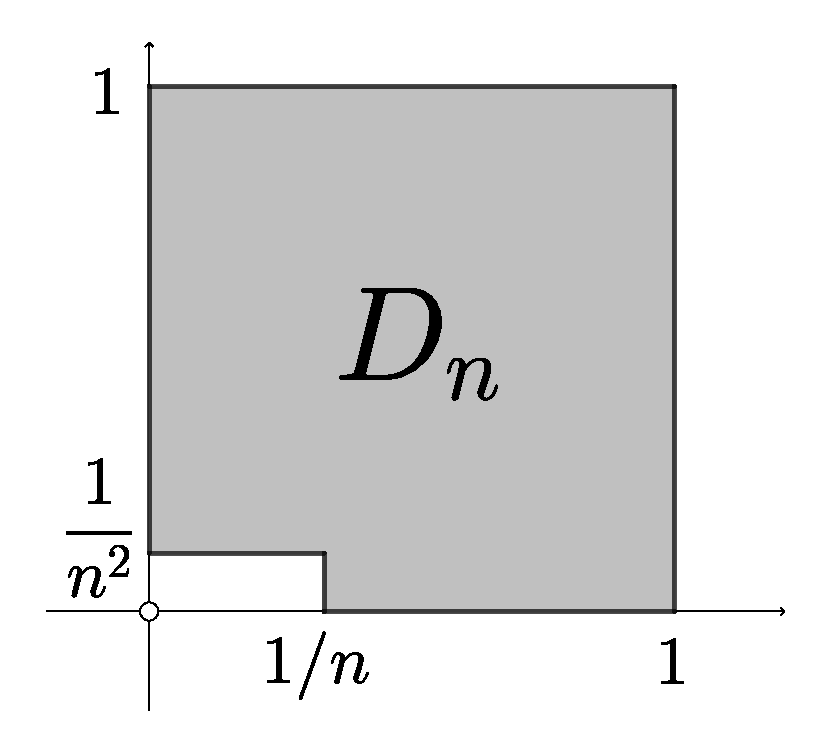
\includegraphics[width=4.8cm]{10/rowlong.pdf}&
     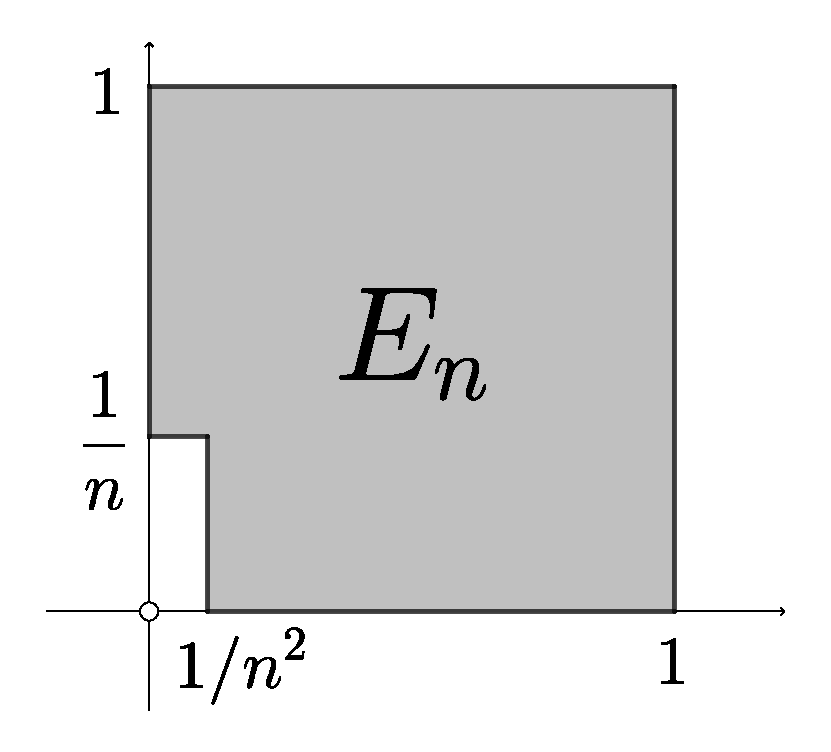
\includegraphics[width=4.8cm]{10/collong.pdf}\\
     $D_n = D-\left( \left[0, \frac{1}{n}\right) \times \left[0, \frac{1}{n^2}\right) \right)$ &
     $E_n = D-\left( \left[0, \frac{1}{n^2}\right) \times \left[0, \frac{1}{n}\right) \right)$
   \end{tabular}
 \end{figure}
 
 このとき,以下のように増加近似列の選び方によって極限値が異なる.
 \begin{align*}
   \iint_{D_n} \frac{x-y}{(x+y)^3}\ dx dy 
   &= \int_{0}^{\frac{1}{n}}\left( \int_{\frac{1}{n^2}}^{1}\frac{x-y}{(x+y)^3}\ dy \right) dx 
     + \int_{\frac{1}{n}}^{1}\left( \int_{0}^{1}\frac{x-y}{(x+y)^3}\ dy \right) dx\\[1ex]
   &= \int_{0}^{\frac{1}{n}}\left[\frac{y}{(x+y)^2}\right]_{y=\frac{1}{n^2}}^{y=1}\ dx 
     + \int_{\frac{1}{n}}^{1} \left[ \frac{y}{(x+y)^2}\right]_{y=0}^{y=1}\ dx\\[1ex]
   &= \int_{0}^{\frac{1}{n}}\left( \frac{1}{(x+1)^2} - \frac{1/n^2}{(x+1/n^2)^2}\right) dx 
   + \int_{\frac{1}{n}}^{1} \frac{dx}{(x+1)^2}\\[1ex]
   &= \frac{1}{2} - \frac{1}{1+1/n} \to -\frac{1}{2} \; (n \to \infty)\\[1ex]
   \iint_{E_n} \frac{x-y}{(x+y)^3}\ dx dy
   &=\int_{0}^{\frac{1}{n^2}}\left( \int_{\frac{1}{n}}^{1}\frac{x-y}{(x+y)^3}\ dy \right) dx
     + \int_{\frac{1}{n^2}}^{1}\left( \int_{0}^{1}\frac{x-y}{(x+y)^3}\ dy \right) dx\\[1ex]
   &=\int_{0}^{\frac{1}{n^2}}\left[ \frac{y}{(x+y)^2}\right]_{y=\frac{1}{n}}^{1}\ dx
     + \int_{\frac{1}{n^2}}^{1} \left[ \frac{y}{(x+y)^2}\right]_{y=0}^{y=1}\ dx\\[1ex]
   &=\int_{0}^{\frac{1}{n^2}}\left( \frac{1}{(x+1)^2} - \frac{1/n}{(x+1/n)^2}\right) dx
     + \int_{\frac{1}{n^2}}^{1}\frac{dx}{(x+1)^2}\ dx\\[1ex]
   &= \frac{1}{2} - \frac{1}{n+1} \to \frac{1}{2} \; (n \to \infty)
 \end{align*}
 これより広義積分 $\ds \iint_{D} \frac{x-y}{(x+y)^3}\ dx dy$ は発散す
 る.
 \newpage
 
 先程の例のように,広義2重積分
 \begin{equation}\label{eq:improper-int}
   \iint_{D} f(x,y) \ dx dy
 \end{equation}
 において,$D$ で $f(x,y)>0$ となることも $f(x,y)<0$ となることもある場
 合は定理\ref{thm:improper-conv}は使えず,1個の増加近似列に関する極限を
 調べるだけでは不十分であり,あらゆる増加近似列に対して同じ極限値に収束
 するかどうかを調べる必要がある.このような場合は,まず被積分関数 $f$ に対して
 \begin{equation}\label{eq:f_pm}
   f_{+}(x,y) := \left\{
     \begin{array}{cl}
       f(x,y) & \left( f(x,y) \geqq 0 \right)\\[1ex]
       0 & \left( f(x,y) \leqq 0\right)
     \end{array}
   \right. \qquad
   f_{-}(x,y) := \left\{
     \begin{array}{cl}
       0 & \left( f(x,y) \geqq 0\right)\\[1ex]
       -f(x,y) & \left( f(x,y) \leqq 0 \right)
     \end{array}
   \right.
 \end{equation}
 として,$f(x,y)$ を
 \[
   f(x,y) = f_{+}(x,y) - f_{-}(x,y)
 \]
 と分ける.$D$ 上で $f_{+}(x,y)\geqq 0 , \; f_{-}(x,y) \geqq 0$ なので,
 定理\ref{thm:improper-conv}から広義2重積分
 \begin{equation}\label{eq:improper-pm}
   \iint_{D}f_{+}(x,y) \ dxdy, \qquad \iint_{D}f_{-}(x,y) \ dxdy
 \end{equation}
 の収束・発散はそれぞれ $D$ の1個の増加近似列について極限を調べればよい.
 これらのいずれもが収束するとき,広義2重積分 (\ref{eq:improper-int}) は
 収束し,以下が成り立つ.
 \[
   \iint_{D} f(x,y) \ dx dy = \iint_{D}f_{+}(x,y) \ dx dy - \iint_{D} f_{-}(x,y) \ dx
 \]
 一方,(\ref{eq:improper-pm})のどちらか一方でも発散すれば広義
 積分 (\ref{eq:improper-int}) は発散する.以上を定理としてまとめる.

 \begin{theorem}\label{thm:improper-criterion} 広義2重積分
   $\ds \iint_{D} f(x,y) \ dxdy$ の収束に関して次が成り立つ.
   \[
     \iint_{D} f(x,y) \ dx dy \text{ は収束する } \quad
     \Longleftrightarrow \quad \iint_{D}f_{+}(x,y) \ dxdy, \; \iint_{D}f_{-}(x,y) \ dxdy \text{ が
       共に収束する}
   \]
   さらに,広義2重積分 $\ds \iint_{D}f(x,y) \ dxdy$ が収束するとき,以下が成り立つ.
   \[
     \iint_{D}f(x,y) \ dx dy = \iint_{D}f_{+}(x,y) \ dxdy - \iint_{D} f_{-}(x,y) \ dxdy
   \]
 \end{theorem}

 なお,広義2重積分の収束・発散を判定するのみであれば,次の定理を根拠として $|f(x,y)|$ の広義
 2重積分の収束・発散を定理\ref{thm:improper-conv}を使って判定してもよい.

 \begin{theorem}
   広義2重積分 $\ds \iint_{D} f(x,y) \ dxdy$ の収束に関して次が成り立つ.
   \[
     \iint_{D}f(x,y) \ dx dy \text{ は収束する } \quad
     \Longleftrightarrow \quad \iint_{D}|f(x,y)| \ dxdy \text{ は収束する }
   \]
   特に,広義2重積分 $\ds \iint_{D}|f(x,y)| \ dxdy$ が収束するとき,以下が成り立つ.
   \[
     \iint_{D} |f(x,y)| \ dxdy = \iint_{D} f_{+}(x,y) \ dx dy + \iint_{D} f_{-}(x,y) \ dxdy
   \]
 \end{theorem}
 
 前々ページで例として挙げた,以下の広義2重積分の収束・発散を定理\ref{thm:improper-criterion}を使っ
 て判定してみる.
 \[
   \iint_{D} \frac{x-y}{(x+y)^3} \ dx dy \qquad D=\Set{(x,y) \ \mid \
     0 \leqq x \leqq 1, \; 0 \leqq y \leqq 1, \; (x,y) \neq (0,0)}
 \]
 被積分関数に $f(x,y)$ と名前をつければ,(\ref{eq:f_pm}) の $f_{+}, f_{-}$ はそれぞれ
 \[
   f_{+}(x,y) = \left\{
     \begin{array}{cl}
       \dfrac{x-y}{(x+y)^3} & ( x \geqq y)\\[1ex]
       0 & ( x \leqq y)
     \end{array}
   \right. \qquad f_{-}(x,y) = \left\{
     \begin{array}{cl}
       0 & (x \geqq y)\\[1ex]
       -\dfrac{x-y}{(x+y)^3} & (x \leqq y)
     \end{array}
   \right.
 \]
 である.そこで,
 \[
   D^{+}:= D \cap \Set{(x,y) \ \mid \ x \geqq y}  \qquad D^{-}:= D \cap \Set{(x,y) \ \mid \ x \leqq y}
 \]
 とすれば,$\ds D = D^{+} \cup D^{-}$ であり,$D^{+} \cap D^{-}$ の面積は $0$ なので
 \[
   \begin{aligned}
     \iint_{D} f^{+}(x,y) \ dxdy &= \iint_{D^{+}} \frac{x-y}{(x+y)^3} \ dxdy + \iint_{D^{-}} 0 \ dx dy
                                   = \iint_{D^{+}} f(x,y) \ dxdy\\[1ex]
     \iint_{D} f^{-}(x,y) \ dxdy &= \iint_{D^{+}} 0 \ dxdy  + \iint_{D^{-}} -\frac{x-y}{(x+y)^3} \ dxdy
                                   = -\iint_{D^{-}} f(x,y) \ dxdy
   \end{aligned}
 \]
 である.従って,$D^{+}, D^{-}$ 上での $f(x,y)$ の広義2重積分の収束・発
 散を調べればよい.\\

 まず,$D^{+}$ 上での $f(x,y)$ の広義2重積分の収束・発散を調べる.$D^{+}$ 上で $f(x,y) \geqq 0$ であり,
 \[
   D^{+}_{n} := \Set{(x,y) \ | \ \frac{1}{n} \leqq x \leqq
     1, \; 0 \leqq y \leqq x} \; (n \geqq 2)
 \]
 とすれば $\Set{D^{+}_n}$ は $D^{+}$ の増加近似列なので,定理\ref{thm:improper-conv}から極限
 \[
   \lim_{n \to \infty} \iint_{D^{+}_{n}} \frac{x-y}{(x+y)^3} \ dxdy
 \]
 が収束するか $+\infty$ に発散するかを判定すればよい.
 \[
   \begin{aligned}
     \iint_{D^{+}_n} f(x,y) \ dxdy
     &= \int_{\frac{1}{n}}^{1} \left( \int_{0}^{x} \frac{x-y}{(x+y)^3} \ dy \right) dx
       = \int_{\frac{1}{n}}^{1}\left[ \frac{y}{(x+y)^2}\right]_{y=0}^{y=x} \ dx
       = \int_{\frac{1}{n}}^{1} \frac{dx}{4x}\\[1ex]
     & = \frac{\log n}{4} \to +\infty \; (n \to \infty)
   \end{aligned}
 \]
 なので,広義2重積分 $\ds \iint_{D^{+}} f(x,y) \ dxdy$ は発散する.よっ
 て,$D^{-}$ 上の広義2重積分を調べるまでもなく,定理\ref{thm:improper-criterion}から広義2重積分
 $\ds \iint_{D} \frac{x-y}{(x+y)^3} \ dxdy$ は発散することがわかる.\\

 ちなみに,$D^{-}$ 上の広義2重積分 $\ds \iint_{D^{-}} f(x,y) \
 dxdy$ も $+\infty$ に発散することが同様の計算で確かめられる.



\end{document}
